\documentclass[dvisvgm]{standalone}

\usepackage{tikz}
\usetikzlibrary {arrows, positioning, automata}

\begin{document}

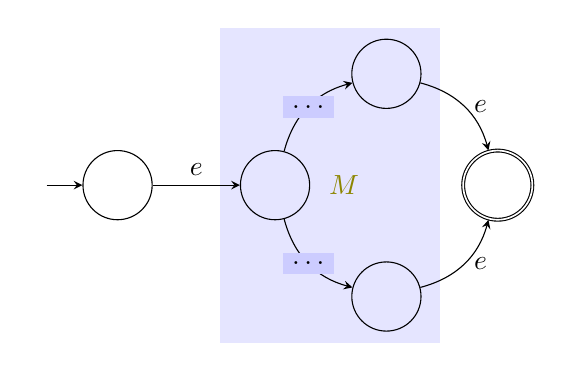
\begin{tikzpicture}[
    ->,
    >=stealth,
    node distance=2cm,
    initial text=$ $,
    on grid,
]

    \node[rectangle, text = olive, fill = blue!10!white, minimum width = 2.8cm, minimum height = 4cm] (M1) at (0.7, 0) {$\ \ \ M$};

    \node[           state]                    (A) {};
    \node[initial,   state, left =of A]        (Q) {};
    \node[           state, above right =of A] (B) {};
    \node[           state, below right =of A] (C) {};
    \node[accepting, state, above right =of C] (D) {};

    \path
        (Q) edge [above]           node                {$e$}      (A)
        (A) edge [bend left]       node [fill=blue!20] {$\dots$}  (B)
        (A) edge [bend right]      node [fill=blue!20] {$\dots$}  (C)
        (B) edge [right, bend left]       node                {$e$}      (D)
        (C) edge [right, bend right]      node                {$e$}      (D)
    ;
\end{tikzpicture}

\end{document}